% Options for packages loaded elsewhere
\PassOptionsToPackage{unicode}{hyperref}
\PassOptionsToPackage{hyphens}{url}
%
\documentclass[
  a4paper,
]{article}
\usepackage{amsmath,amssymb}
\usepackage{lmodern}
\usepackage{ifxetex,ifluatex}
\ifnum 0\ifxetex 1\fi\ifluatex 1\fi=0 % if pdftex
  \usepackage[T1]{fontenc}
  \usepackage[utf8]{inputenc}
  \usepackage{textcomp} % provide euro and other symbols
\else % if luatex or xetex
  \usepackage{unicode-math}
  \defaultfontfeatures{Scale=MatchLowercase}
  \defaultfontfeatures[\rmfamily]{Ligatures=TeX,Scale=1}
\fi
% Use upquote if available, for straight quotes in verbatim environments
\IfFileExists{upquote.sty}{\usepackage{upquote}}{}
\IfFileExists{microtype.sty}{% use microtype if available
  \usepackage[]{microtype}
  \UseMicrotypeSet[protrusion]{basicmath} % disable protrusion for tt fonts
}{}
\makeatletter
\@ifundefined{KOMAClassName}{% if non-KOMA class
  \IfFileExists{parskip.sty}{%
    \usepackage{parskip}
  }{% else
    \setlength{\parindent}{0pt}
    \setlength{\parskip}{6pt plus 2pt minus 1pt}}
}{% if KOMA class
  \KOMAoptions{parskip=half}}
\makeatother
\usepackage{xcolor}
\IfFileExists{xurl.sty}{\usepackage{xurl}}{} % add URL line breaks if available
\IfFileExists{bookmark.sty}{\usepackage{bookmark}}{\usepackage{hyperref}}
\hypersetup{
  pdftitle={Sensorimotor Learning of a Virtual Skill},
  pdfauthor={Spencer R. Wilson},
  hidelinks,
  pdfcreator={LaTeX via pandoc}}
\urlstyle{same} % disable monospaced font for URLs
\usepackage[margin=30mm]{geometry}
\usepackage{graphicx}
\makeatletter
\def\maxwidth{\ifdim\Gin@nat@width>\linewidth\linewidth\else\Gin@nat@width\fi}
\def\maxheight{\ifdim\Gin@nat@height>\textheight\textheight\else\Gin@nat@height\fi}
\makeatother
% Scale images if necessary, so that they will not overflow the page
% margins by default, and it is still possible to overwrite the defaults
% using explicit options in \includegraphics[width, height, ...]{}
\setkeys{Gin}{width=\maxwidth,height=\maxheight,keepaspectratio}
% Set default figure placement to htbp
\makeatletter
\def\fps@figure{htbp}
\makeatother
\setlength{\emergencystretch}{3em} % prevent overfull lines
\providecommand{\tightlist}{%
  \setlength{\itemsep}{0pt}\setlength{\parskip}{0pt}}
\setcounter{secnumdepth}{5}

%% pandoc-fignos: required package
\usepackage[capitalise]{cleveref}
\ifluatex
  \usepackage{selnolig}  % disable illegal ligatures
\fi

\title{Sensorimotor Learning of a Virtual Skill}
\author{Spencer R. Wilson}
\date{\today}

\usepackage[capitalise]{cleveref}
\usepackage{graphicx}
\graphicspath{{/Users/spencerw/Google Drive/motor_control/phd/}}
\usepackage{subfigure}

\begin{document}
\maketitle

\hypertarget{sec:data}{%
\section{Key Plots}\label{sec:data}}

\begin{figure}
\hypertarget{fig:behavior}{%
\centering
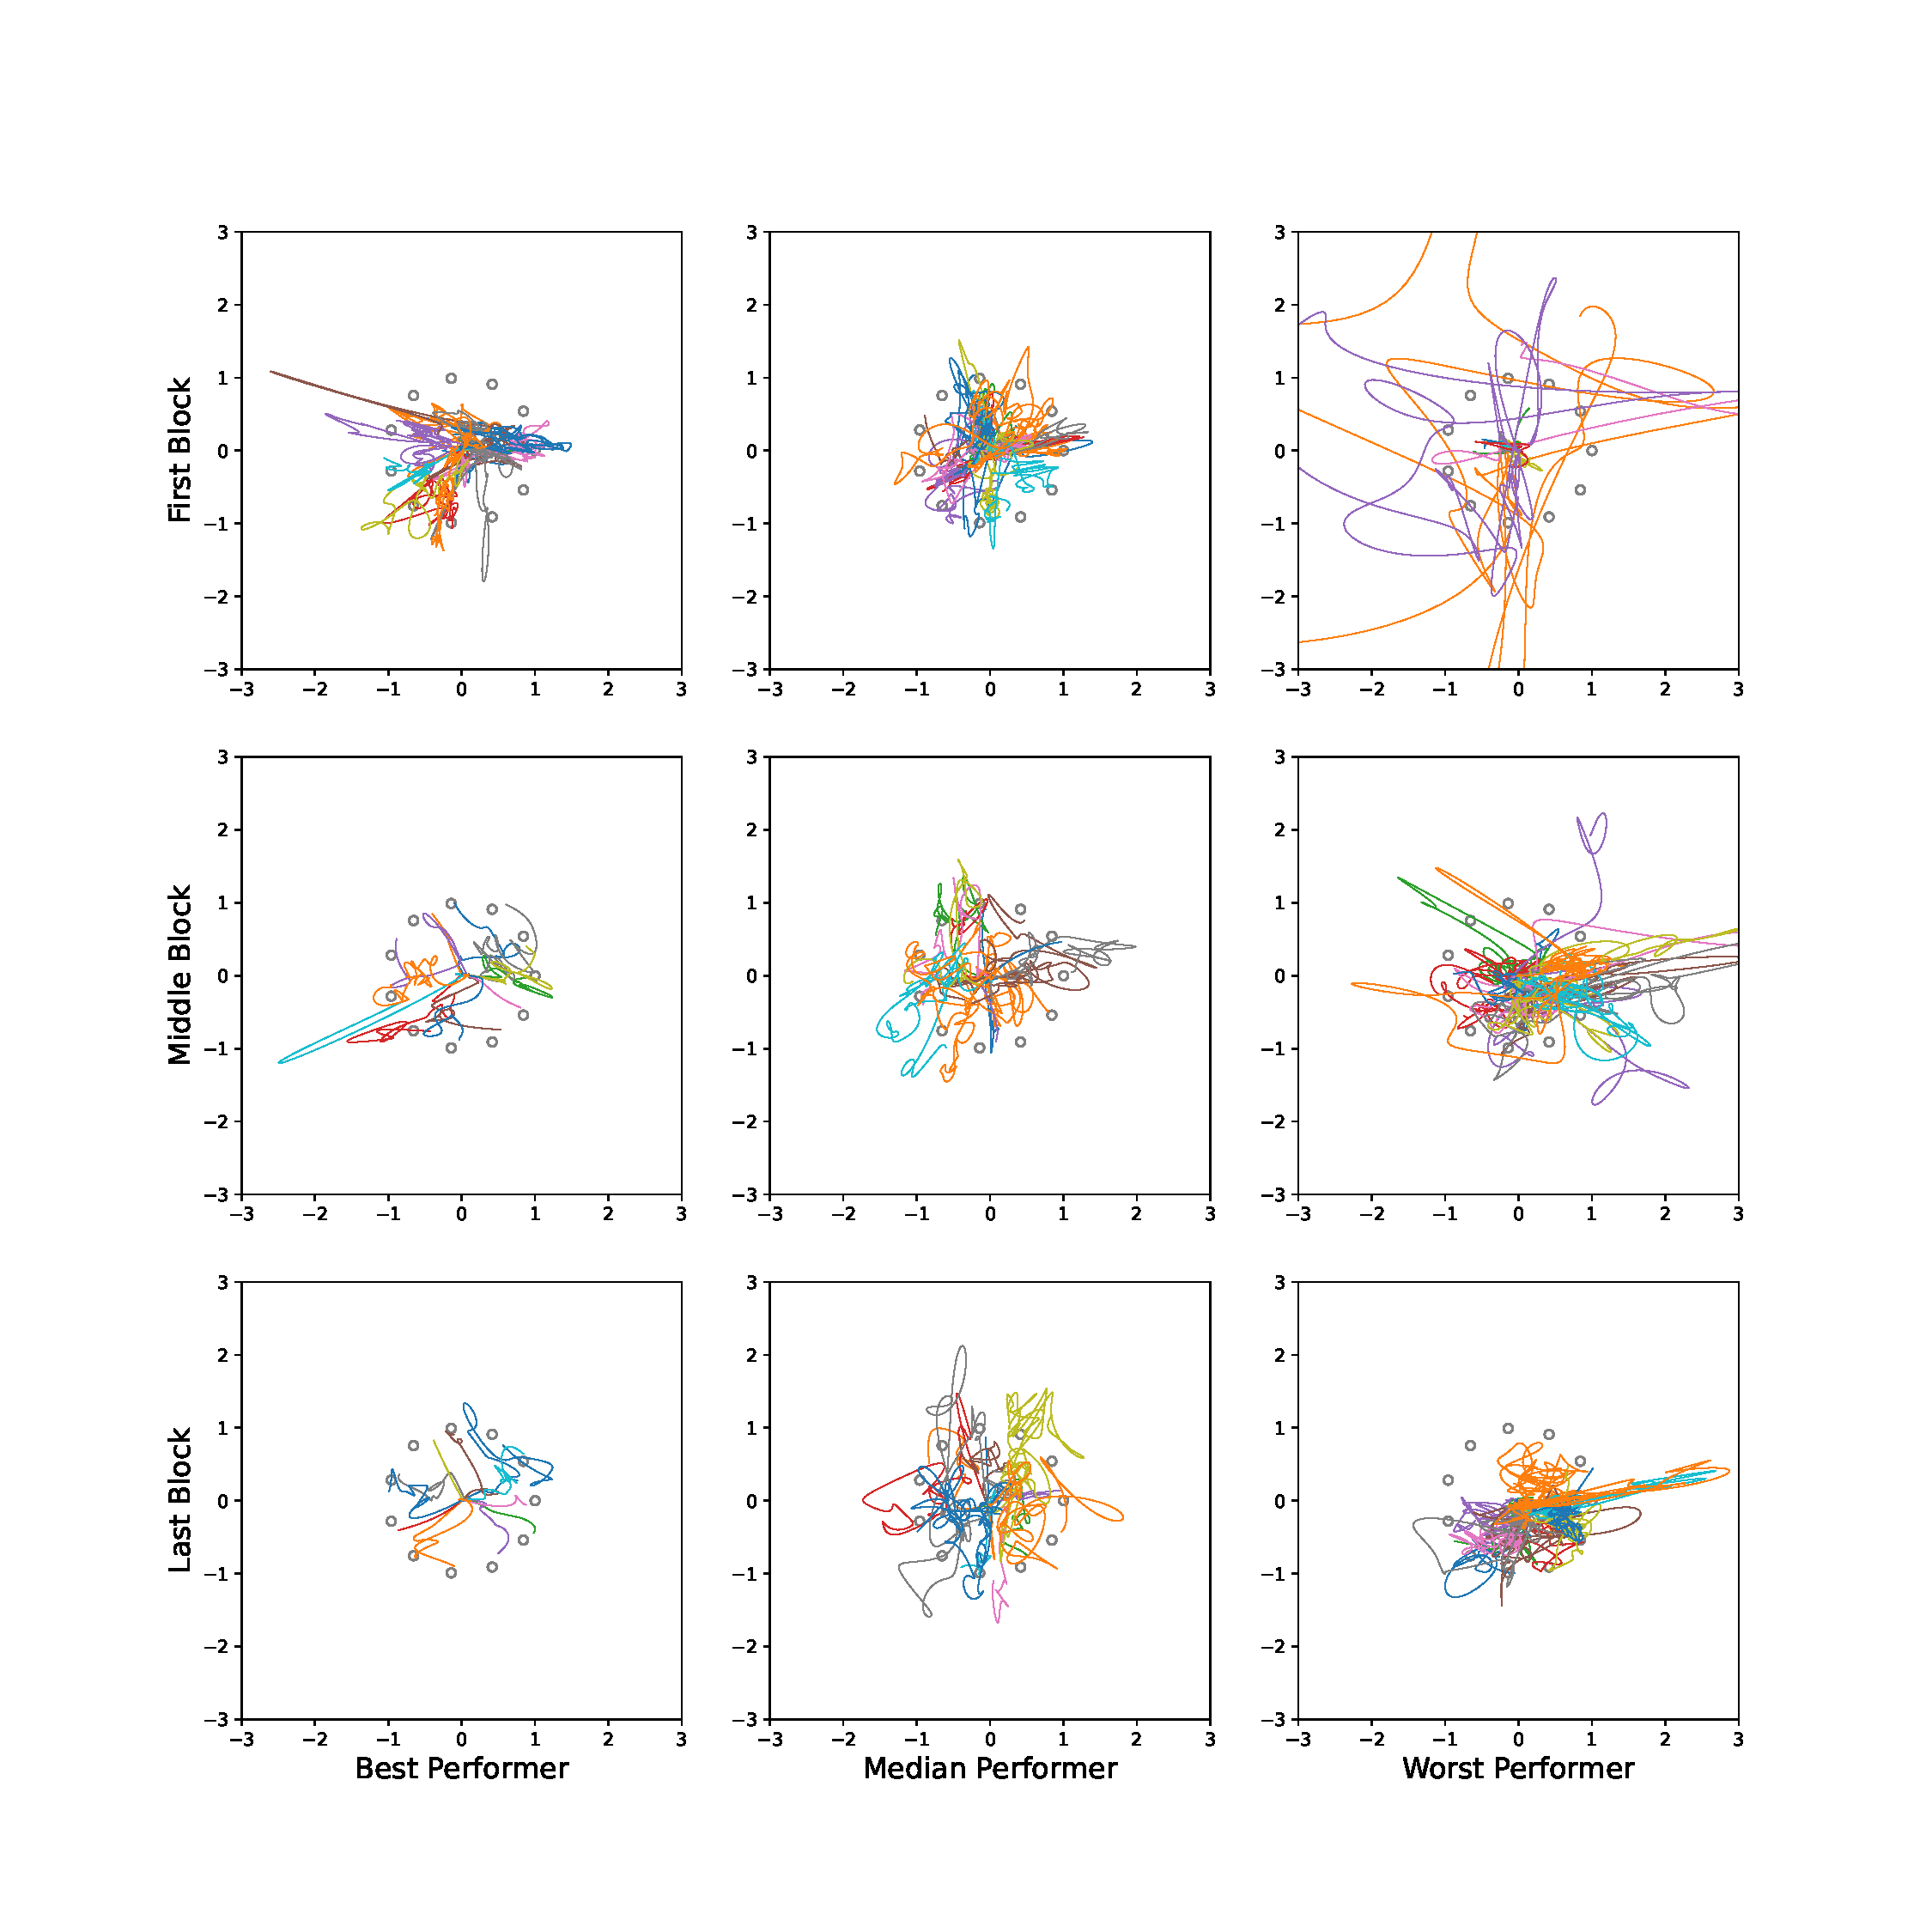
\includegraphics[width=1\textwidth,height=\textheight]{/Users/spencer/motor-control/thesis/sections/../images/data_analysis2023/behavior.pdf}
\caption{Example task behavior. Behavioral trajectories from the
``center hold, reach out'' task. This task required subject to maintain
their cursor in the center of the frame by refraining from any muscle
activity in the recorded forearm for 2s. After this initial period, one
of 12 targets appeared on-screen (shown here as grey circles). The
subject attempted to activate their forearm muscle activity to ``reach''
to each target. Moving their cursor to the target resulted in a ``Hit''.
The cursor was allowed to exit the ``screen'' spanning {[}-2,2{]} as
plotted here, becoming invisible to the subject. Each plot shows cursor
trajectories from a single block of 12 unique targets, each trial a
different color. Each column of three plots is a single subject, from
left to right: the subject with the most, median, and least ``Hits''
across all trials of the task. Each row shows one block of 12 trials,
from top to bottom: the first block, the halfway point, and the last
block.}\label{fig:behavior}
}
\end{figure}

\begin{figure}
\hypertarget{fig:outcomes}{%
\centering
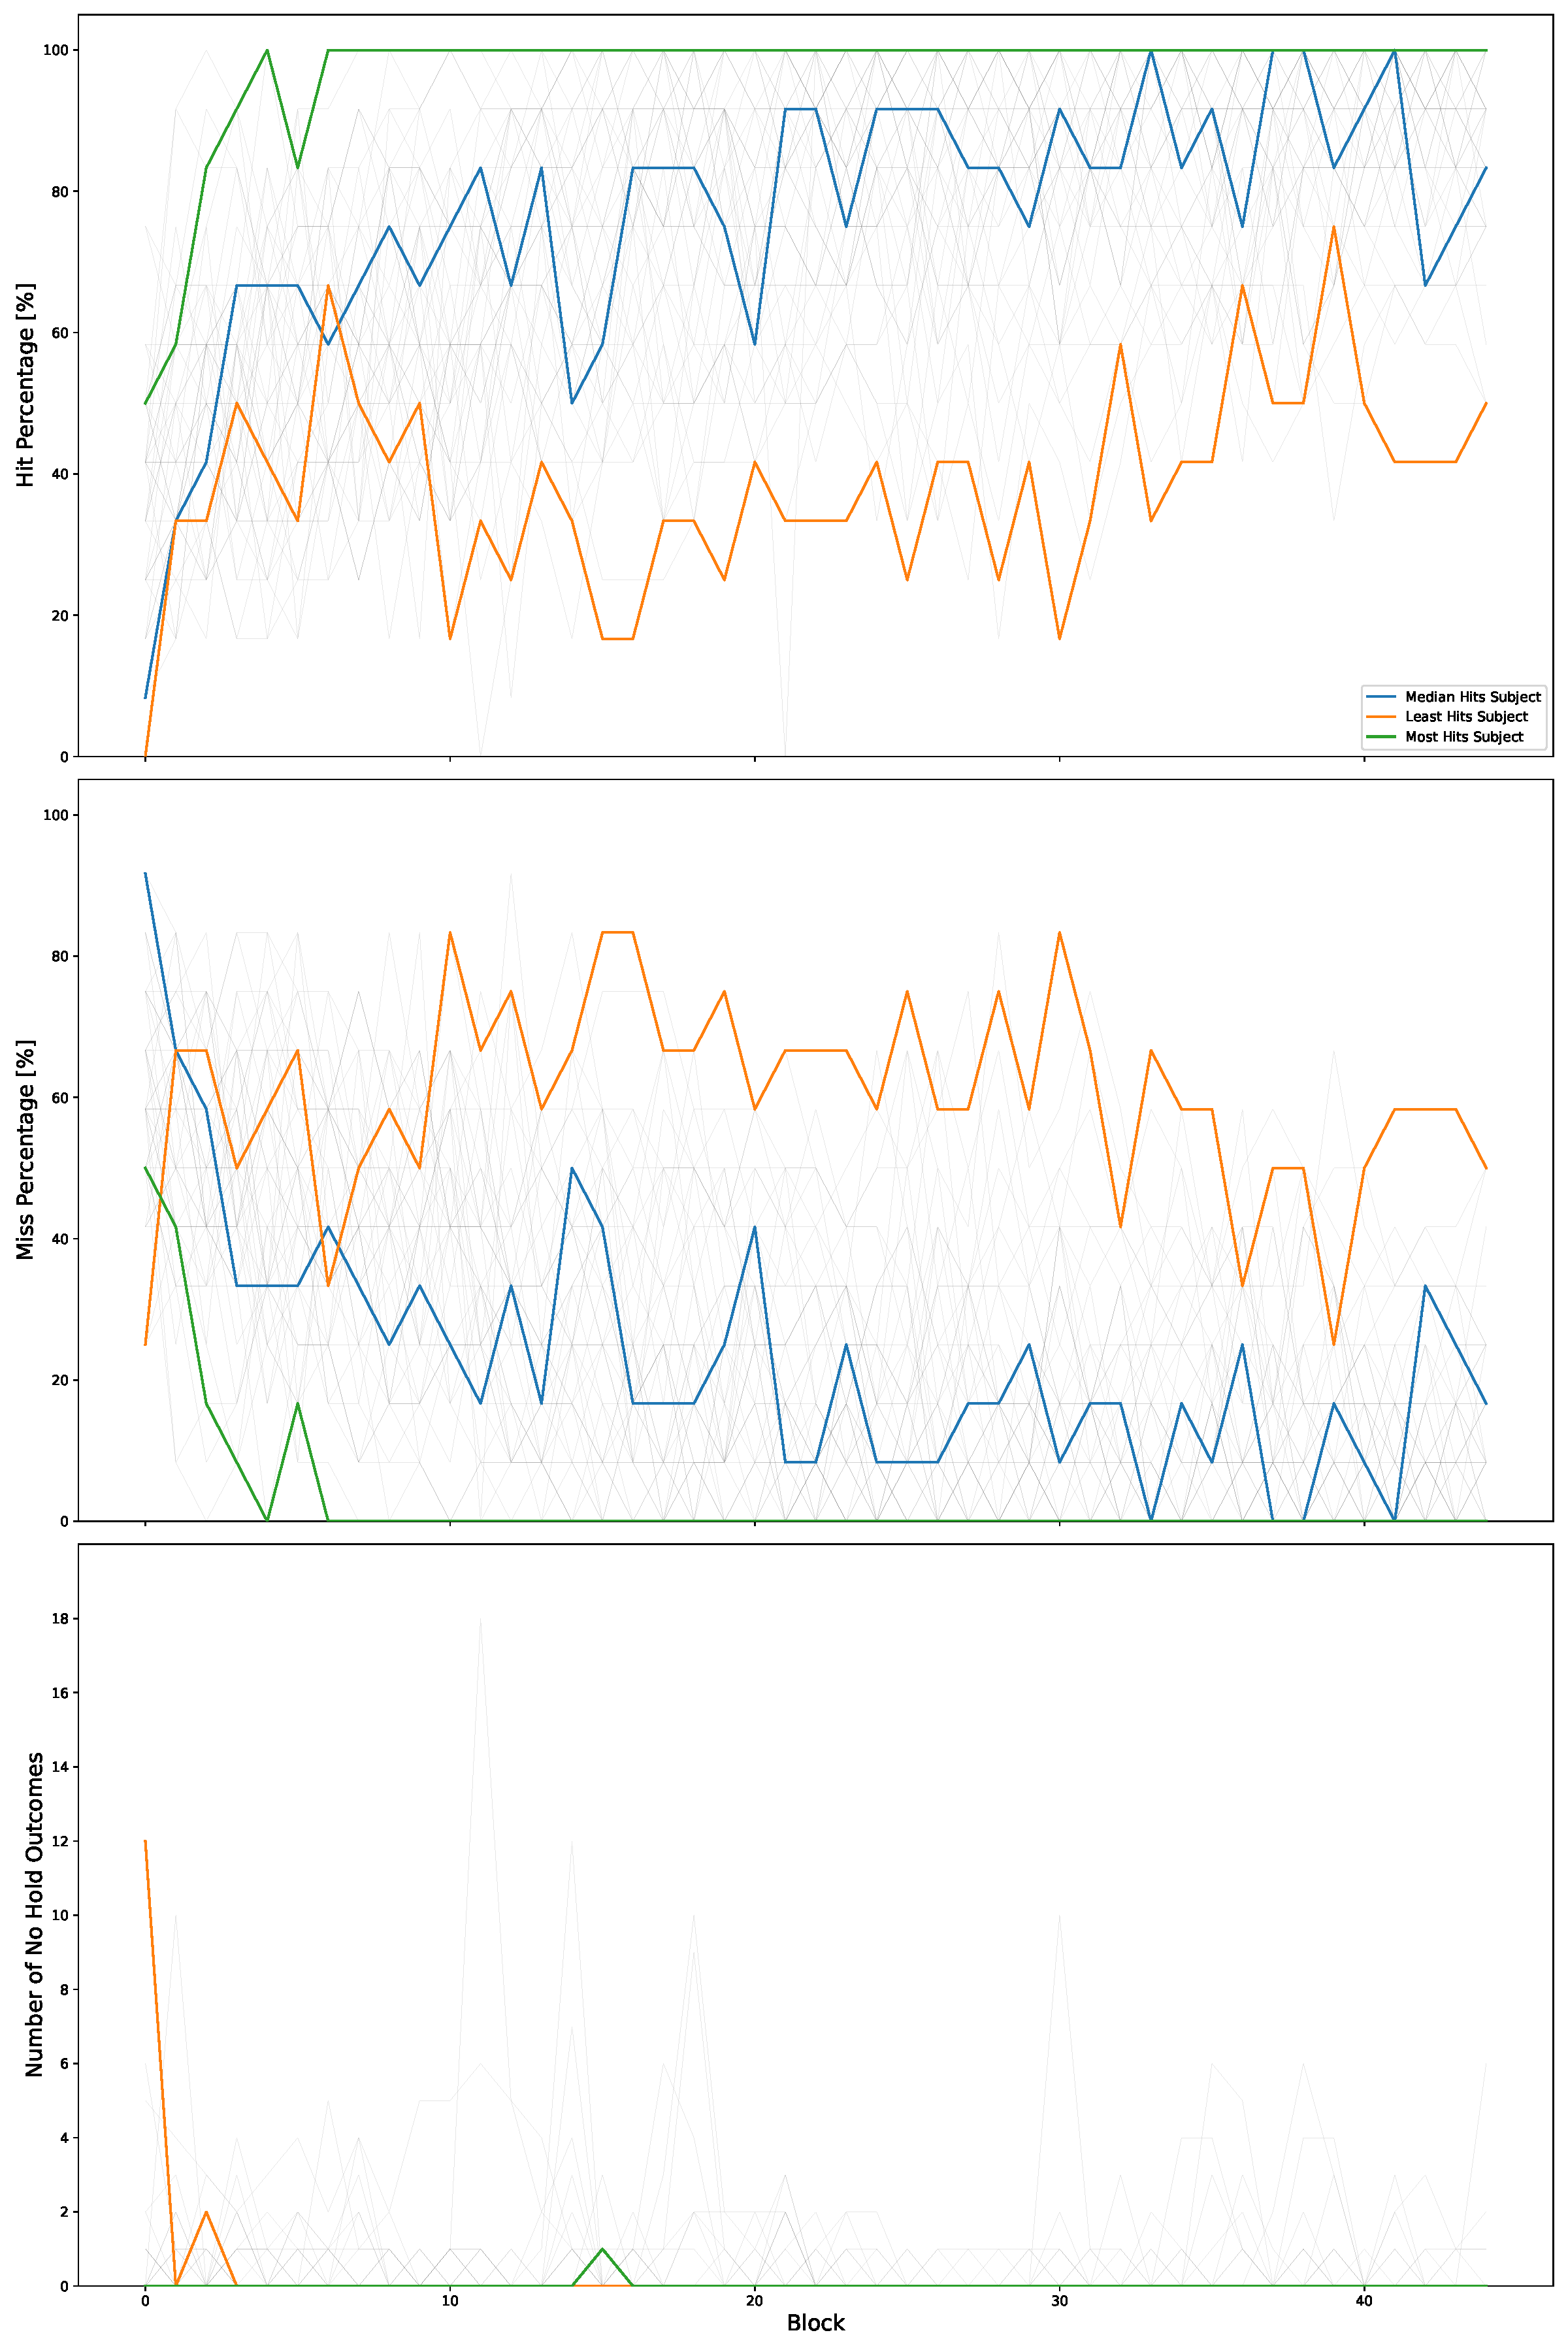
\includegraphics[width=1\textwidth,height=\textheight]{/Users/spencer/motor-control/thesis/sections/../images/data_analysis2023/outcomes.pdf}
\caption{Task outcomes over blocks. Outcomes across all 45 blocks of 12
trials (targets) in the ``center hold, reach out'' task. Subjects with
the most, median, and least hits are shown in green, blue, and orange
respectively. All ofther subjects are show in gray. From top to bottom:
The percentage of ``Hits'' within each block, the percentage of
``Misses'' (timeouts), and ``No Holds'' (subject unable to quiet forearm
muscle activity initially).}\label{fig:outcomes}
}
\end{figure}

\begin{figure}
\hypertarget{fig:decoders}{%
\centering
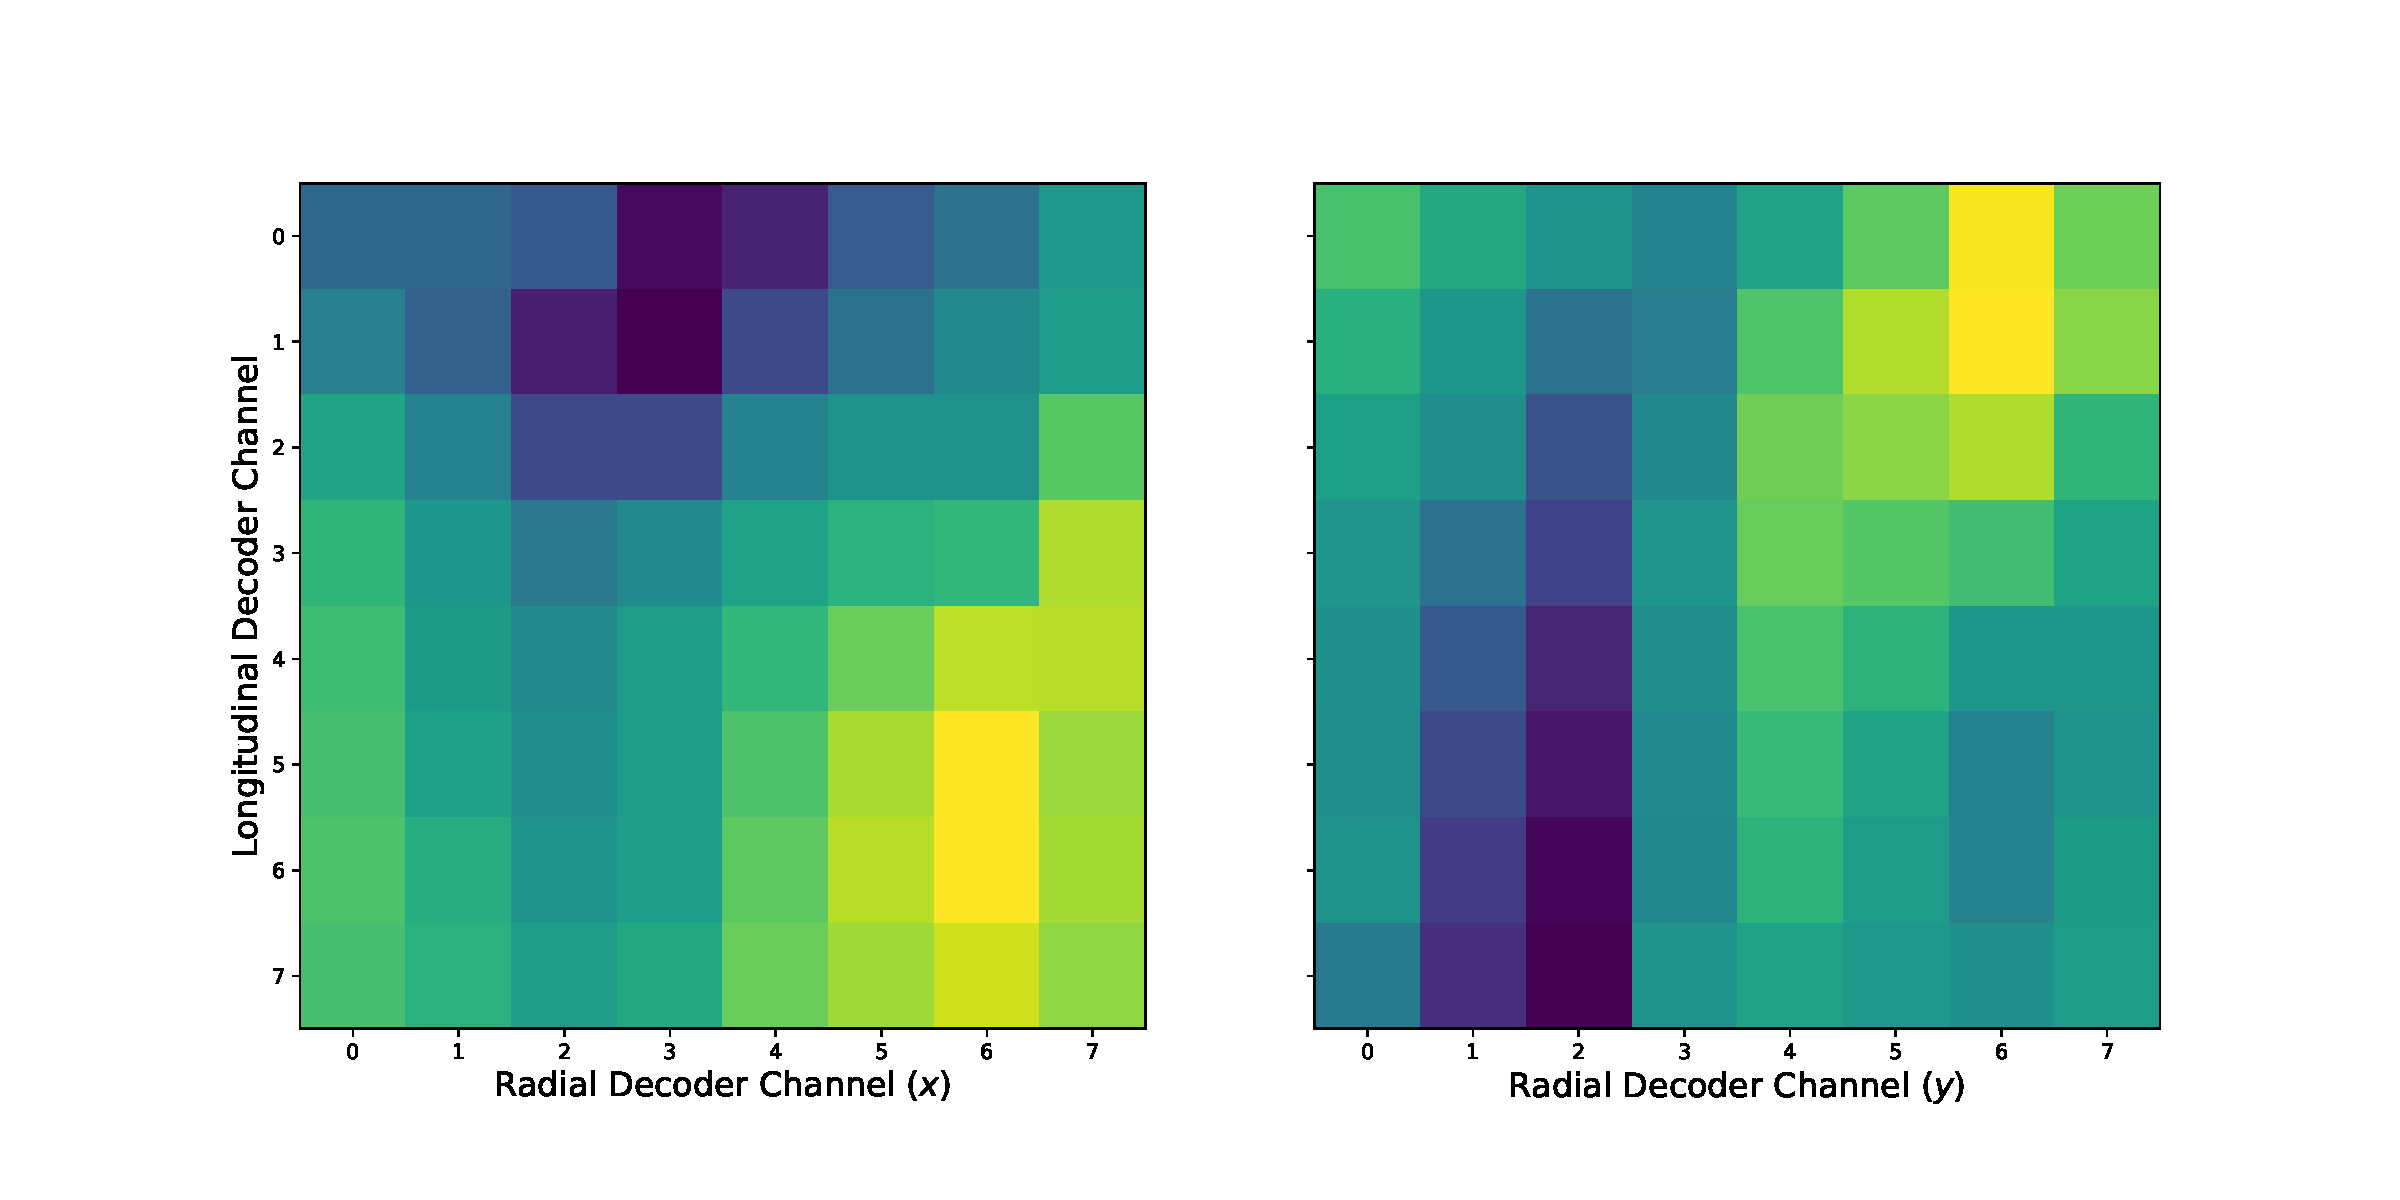
\includegraphics[width=1\textwidth,height=\textheight]{/Users/spencer/motor-control/thesis/sections/../images/data_analysis2023/decoder_heatmap.pdf}
\caption{Example EMG-to-force decoders from a single subject. The
``center hold, reach out'' task works by mapping 64 channels of EMG
activity from subjects' forearms to a 2-dimensional force vector, a
component acting in the \(x\) and \(y\) directions within the task's
linear dynamics. Depicted here are the two 64-dimensional ``decoders''
arranged as the EMG electrodes were arranged on subjects' arms (along
the arm, longitudinally, and around the arm, radially). The left plot
shows the \(x\) force decoder, and the right plot the
\(y\).}\label{fig:decoders}
}
\end{figure}

\begin{figure}
\hypertarget{fig:decoder_correlations}{%
\centering
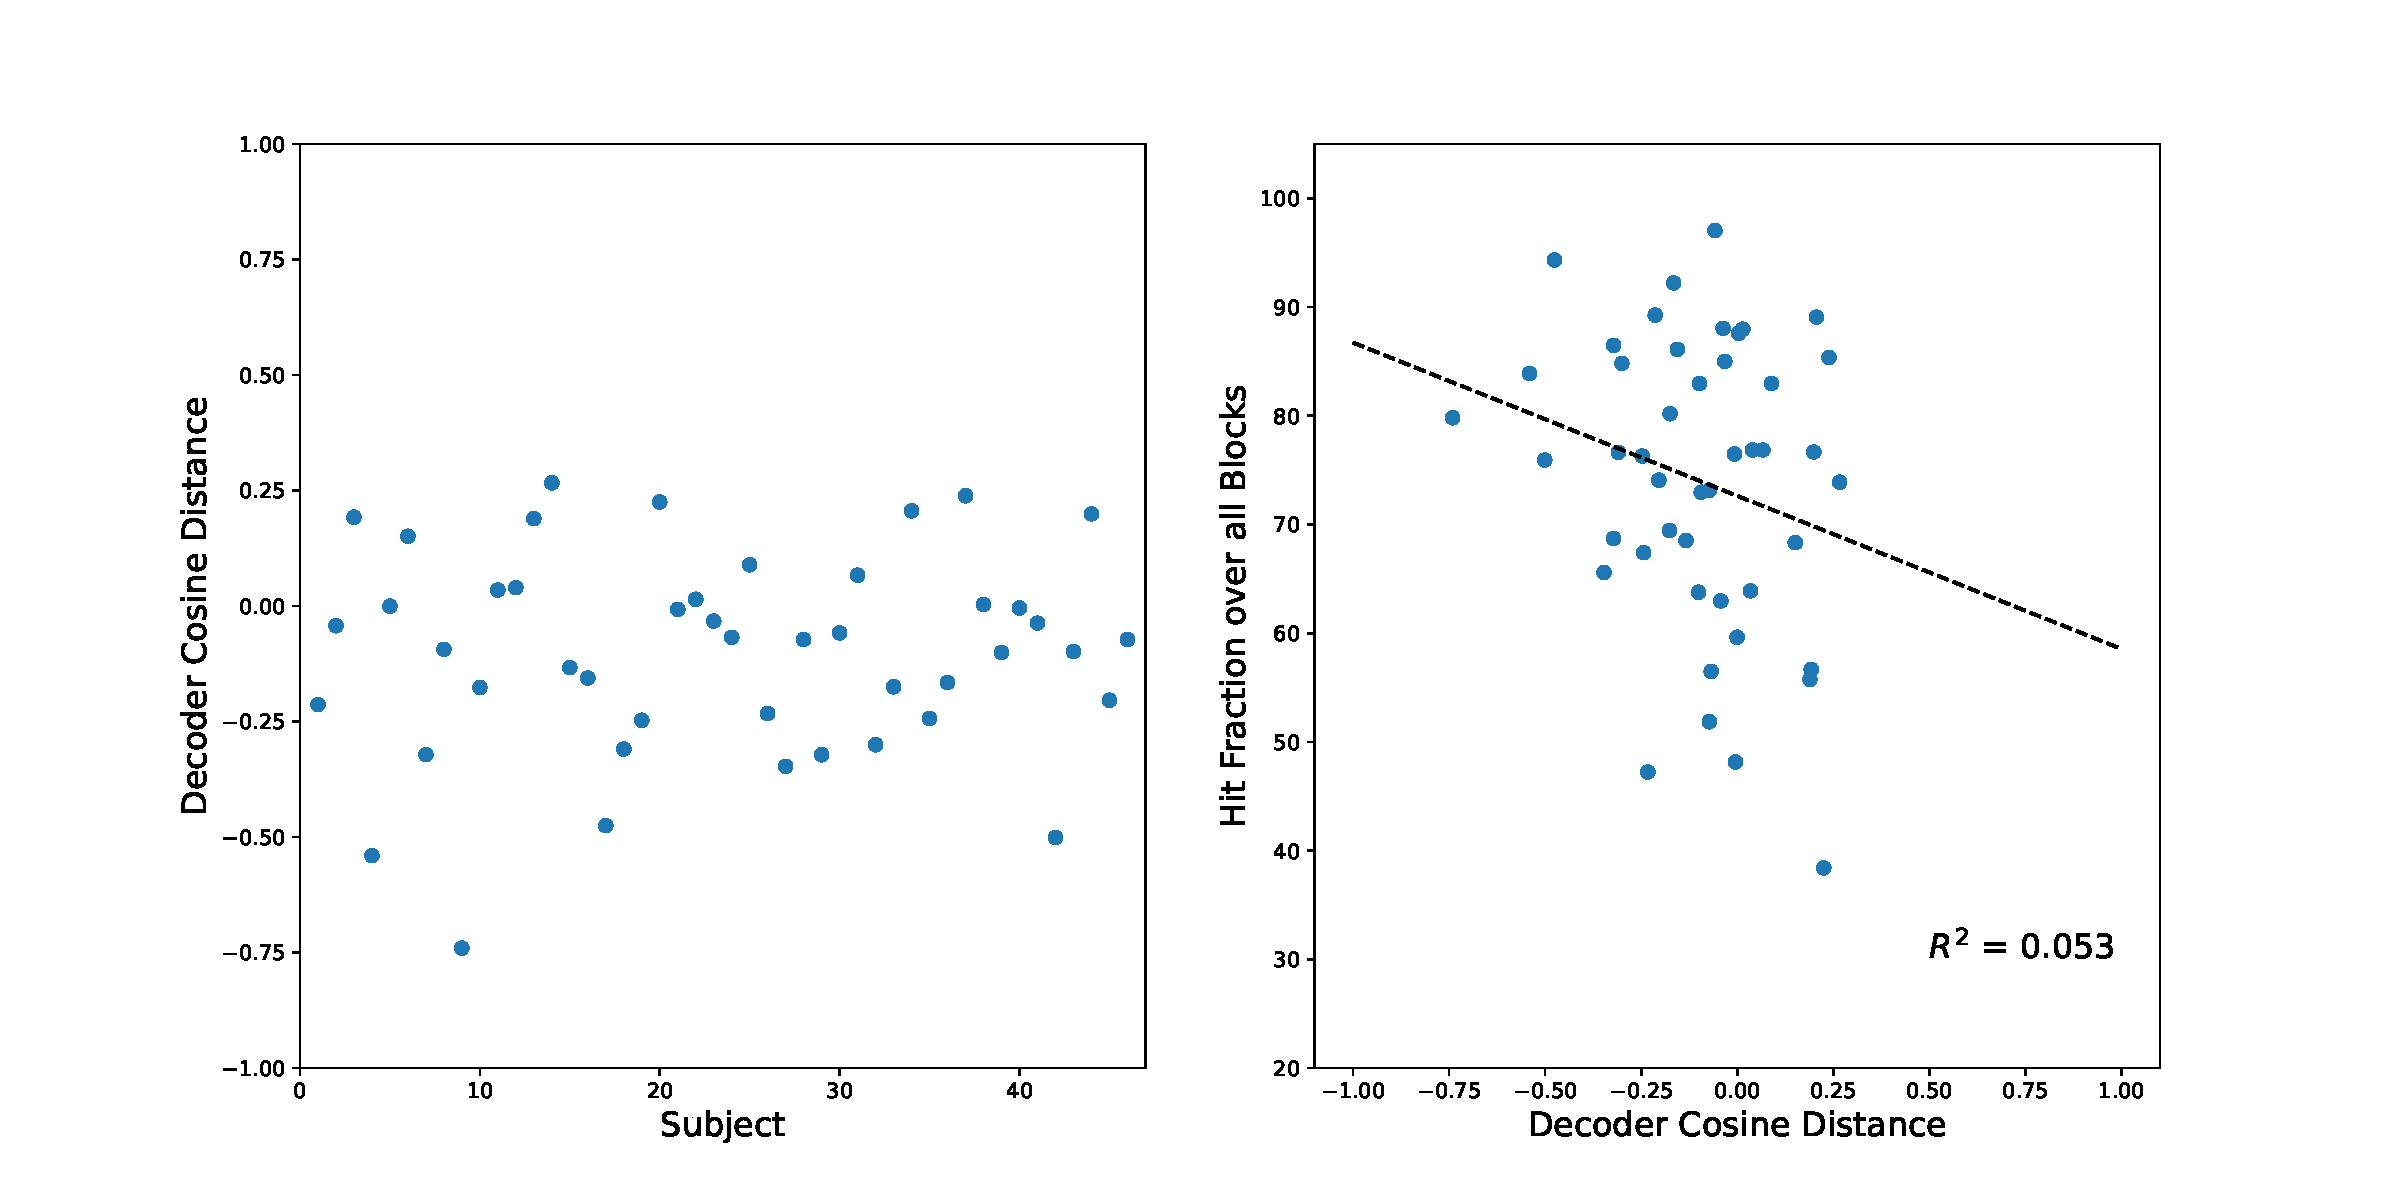
\includegraphics[width=1\textwidth,height=\textheight]{/Users/spencer/motor-control/thesis/sections/../images/data_analysis2023/decoder_correlation.pdf}
\caption{Decoder cosine similarity. EMG-to-force decoders are computed
using a calibration dataset collected before the ``center hold, reach
out'' task. 4 ``modes'' of EMG activity are extracted from the dataset
using non-negative matrix factorization. These 4 modes are then
subtracted in pairs to yield the two 64-dimensional EMG-to-force
mappings, shown in \cref{fig:low_variance_PCs}. The left plot shows the
cosine similarity of the \(x\) and \(y\) EMG-to-force decoders. A cosine
similarity of 1 means the two vectors are parallel, producing identical
forces (in the respective directions) for the same EMG activity
(\(F_x = F_y\)). A cosine similarity of -1 means the vectors are
antiparallel, producing equal but opposite forces in the two directions
(\(F_x = -F_y\)). A cosine similarity of 0 means the decoder directions
are orthogonal; e.g.~producing a force in the \(x\) direction with a
certain EMG activity produces no force in the \(y\) direction. Plotted
across subjects, we see a range of decoder similarities, providing a
variety of task contingencies. The rightmost plot asks whether cosine
similarity is predictive of task success, in terms of the numbers of
``Hits''. We find no significant correlation, implying that the decoder
cosine similarity, in the range we tested, does not predict task
success. Task success, therefore, likely relies on an alternative task
variable.}\label{fig:decoder_correlations}
}
\end{figure}

\begin{figure}
\hypertarget{fig:behavior}{%
\centering
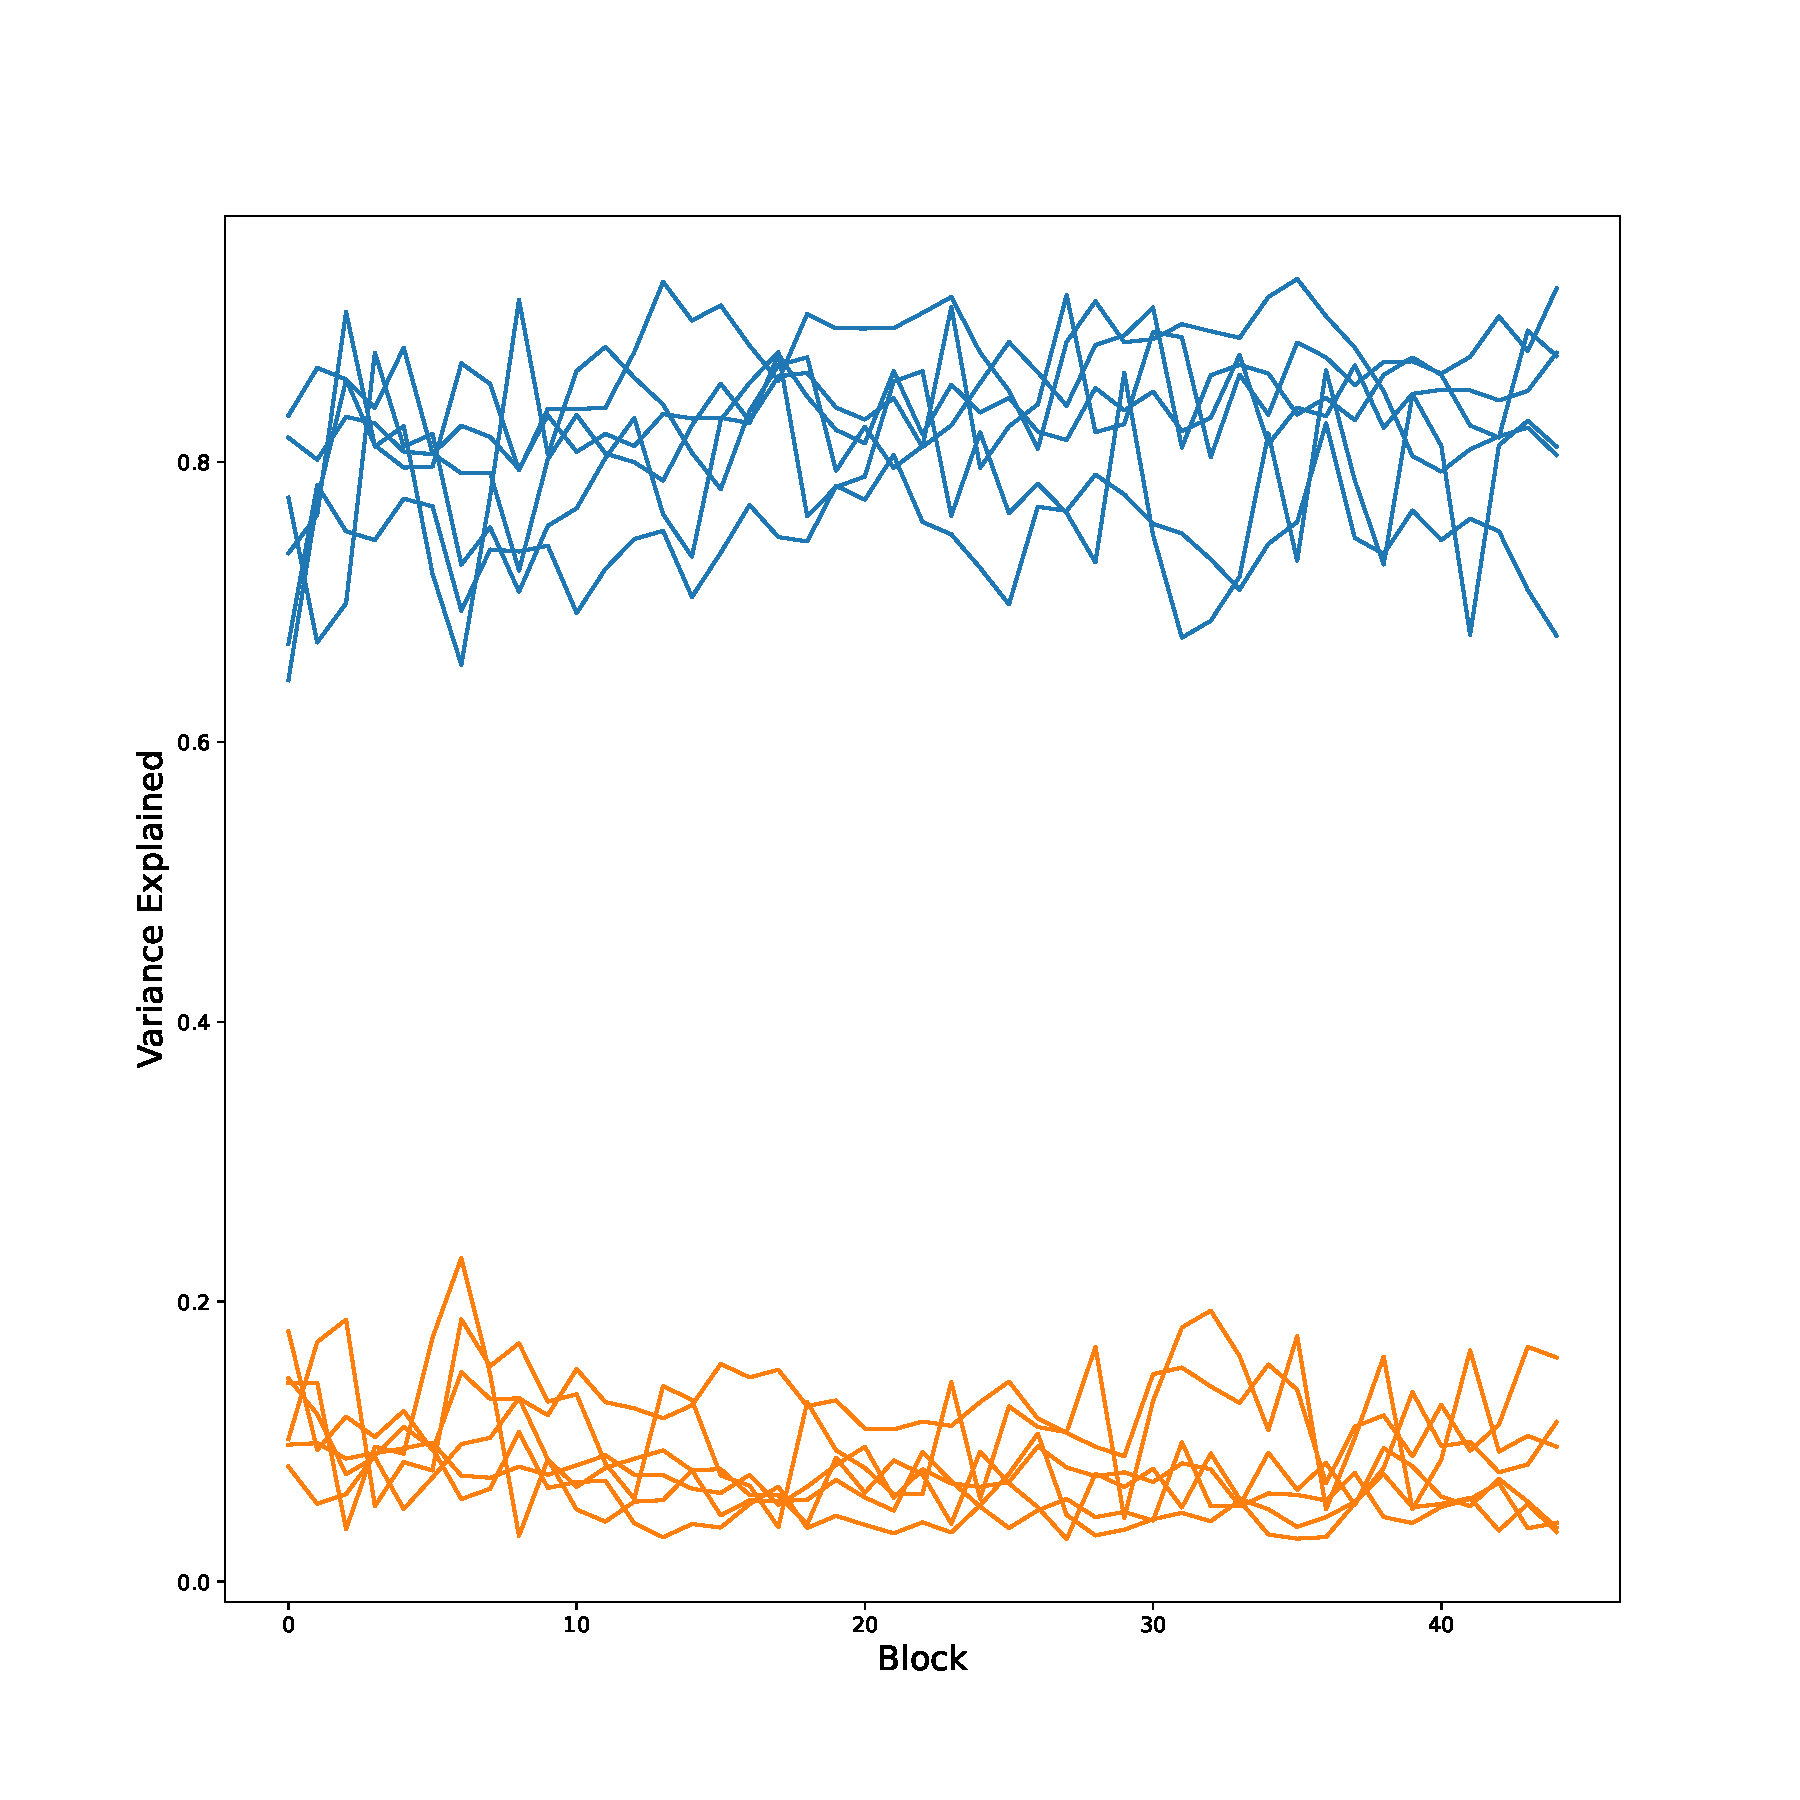
\includegraphics[width=1\textwidth,height=\textheight]{/Users/spencer/motor-control/thesis/sections/../images/data_analysis2023/PCA_blocks.pdf}
\caption{PCA of EMG activity over blocks. The experimental paradigm is
unique in that we have access to the true subject state (EMG activity),
control over the contingency (the decoding from EMG to force in the
task), and the outcome (task behavior). This plot addresses the question
of whether there is a dynamic, over blocks, of the variance of the EMG
signals concatenate over blocks (12 trials). The plot suggests this is
not the case, as the first PCA component of EMG activity, for six
subjects, explains much of the EMG variance for each block, without any
visual indiciation of a trend. This is a common finding, and confirms
what is often found in the literature, that joint and/or muscle
activity, while high-dimensional, displays low dimensional modes.
Exploring the structure of the variance of this signal is a next step,
to understand how subjects manage the variability of their activity to
acheive task success, and how this evolves over
trials.}\label{fig:behavior}
}
\end{figure}

\end{document}
